\PassOptionsToPackage{table}{xcolor}
\documentclass{beamer}

\mode<presentation>
{
  \usetheme{CambridgeUS}      % or try Darmstadt, Madrid, Warsaw, ...
  \usecolortheme{default} % or try albatross, beaver, crane, ...
  \usefonttheme{default}  % or try serif, structurebold, ...
  \setbeamertemplate{navigation symbols}{}
  \setbeamertemplate{caption}[numbered]
} 


\usepackage[spanish]{babel}
\usepackage[utf8x]{inputenc}
\usepackage{algorithm}% http://ctan.org/pkg/algorithms
\usepackage{algpseudocode}% http://ctan.org/pkg/algorithmicx

\title[Subsecuencia Común Más Larga]{Subsecuencia Común Más Larga}
\subtitle[Programación Dinámica]{Programación Dinámica}

\author{Sergio García Prado\\}

\date{10 de Noviembre de 2015}

% Add support for \subsubsectionpage
\def\subsubsectionname{\translate{Subsubsection}}
\def\insertsubsubsectionnumber{\arabic{subsubsection}}
\setbeamertemplate{subsubsection page}
{
  \begin{centering}
    {\usebeamerfont{subsubsection name}\usebeamercolor[fg]{subsubsection name}\subsubsectionname~\insertsubsubsectionnumber}
    \vskip1em\par
    \begin{beamercolorbox}[sep=4pt,center]{part title}
      \usebeamerfont{subsubsection title}\insertsubsubsection\par
    \end{beamercolorbox}
  \end{centering}
}
\def\subsubsectionpage{\usebeamertemplate*{subsubsection page}}

\AtBeginSection{\frame{\sectionpage}}
\AtBeginSubsection{\frame{\subsectionpage}}
\AtBeginSubsubsection{\frame{\subsubsectionpage}}

\begin{document}

%%%%%%%%%%%%%%%

	\begin{frame}
		\titlepage
	\end{frame}

%%%%%%%%%%%%%%%
	
	\begin{frame}
		\tableofcontents
	\end{frame}

%%%%%%%%%%%%%%%

	\section{Introducción}

	
		\subsection{Formulación del Problema}
			\begin{frame}{Formulación del Problema}
 				Dadas dos secuencias de longitud arbitraria, nuestro objetivo es encontrar la subsecuencia común de mayor longitud entre ambas.

			\end{frame}
			
		\subsection{Definiciones}
		
		
			\begin{frame}{Secuencia}

 				\begin{itemize}
			
  					\item Es una colección ordenada de elementos en la cual la repetición está permitida.
  			
					\item Ejemplo: {A, B, C, A, E, F}

				\end{itemize}

			\end{frame}
			
			\begin{frame}{Subsecuencia}

 				\begin{itemize}
			
  					\item Es una secuencia que se obtiene a partir de otra de igual o mayor longitud mediante la supresión de algunos elementos manteniendo el orden de los restantes.
  			
					\item Ejemplo: {A, C, A} es una subsecuencia de {A, B, C, A, E, F}.
  					

				\end{itemize}

			\end{frame}

%%%%%%%%%%%%%%%

	\section{Aplicaciones}

	
		\begin{frame}{Aplicaciones}
 			\begin{itemize}
			
  				\item Secuenciación del ADN.
  			
				\item Software de control de versiones (git).
  					
				\item Comando diff.

			\end{itemize}
		\end{frame}
			
%%%%%%%%%%%%%%%


	\section{Programación Dinámica}

	
		\begin{frame}{Programación Dinámica}
 			\begin{itemize}
			
  				\item Patrón de diseño de algoritmos basado en la división del problema base en subproblemas de menor tamaño y complejidad que solo se resolverán una única vez.
  			
				\item Solapamiento de Problemas.
  					
				\item Subestructura Óptima.

			\end{itemize}
		\end{frame}
	
		\begin{frame}{Solapamiento de Problemas}
 			\begin{itemize}
			
  				\item Un problema tiene esta propiedad si se puede dividir en subproblemas de menor tamaño cuyos resultados se reutilizarán para resolver sucesivos subproblemas de nivel superior.
  			
				\item Ejemplo: Sucesión de Fibonacci.
  					
			\end{itemize}
		\end{frame}
		
		\begin{frame}{Subestructura Óptima}
 			\begin{itemize}
			
  				\item La solución óptima del problema contiene (o depende) de las soluciones óptimas a sus subproblemas..

			\end{itemize}
		\end{frame}
			
%%%%%%%%%%%%%%%

	\section{Subsecuencia Común más larga}

		\subsection{Enfoques Disponibles}
	
			\begin{frame}{Enfoques Disponibles}
 			
				\begin{itemize}
			
					\item N = Cantidad de secuencias.
				
					\item $n_{i} $ = Secuencia i-ésima.

  					\item Boráz: $O(2^{n_{1}}\sum_{i = 2}^{N}n_{i})$.
  			
					\item Programación Dinámica: $O(N\prod_{i = 1}^{N}n_{i})$.
  					
				\end{itemize}
			
			\end{frame}

		\subsection{Enfoque dinámico}
		
			
%%%%%%%%%%%%%%%%
				\begin{frame}{Notación Utilizada}
 			
					\begin{itemize}
			
						\item Se expone el caso de dos secuencias.

						\item $X[0...m-1]$ e $Y[0...n-1]$  secuencias de longitud m y n respectivamente. 	
				
						\item L[0...m][0...n] matriz de tamaño m x n, para almacenar los resultados de cada subproblema.
  					
						\item Sea $S$ una secuencia de longitud $l$  e $i \in (1, l)$, entonces $S_{i}$ es la correspondiente a los $i$ primeros elementos. 
			\newline{}
			Ejemplo: $X = abcde$
			\newline{}
			$X_{1} = a$, $X_{3} = abc$ y $X_{5} = abcde = X$
					\end{itemize}
			
				\end{frame}			

%%%%%%%%%%%%%%%%
			
				\begin{frame}{Fórmula}
 			
					\[
			 		LCS( X_{i}, Y_{j} ) =
						\begin{cases}
				    			0									& \text{if } i = 0 \vee	 j = 0\\
    							LCS( X_{i-1}, Y_{j-1}) + 1					& \text{if } x_{i} = y_{j}\\
    							max(LCS( X_{i}, Y_{j-1}), LCS( X_{i-1}, Y_{j}))	& \text{if } x_{i} \not = y_{j}
						\end{cases}
					\]
			
				\end{frame}

				\begin{frame}{Funcionamiento}
 			
					\begin{itemize}
			
						\item Rellenar matriz L a partir de función LCS.
				
						\item Recorrer L desde $L_{m-1n-1}$ hasta $L_{00}$ guardando los elementos iguales.
  					
					\end{itemize}	
					
				\end{frame}
				
				\begin{frame}{Ejemplo de funcionamiento 1}
 			
					\begin{itemize}
			
						\item X = abcde, m = 5
				
						\item Y = aert, n = 4
  					
					\end{itemize}	
					
				\end{frame}
				
				\begin{frame}{Ejemplo de funcionamiento 2}
 			
\begin{center}
	    		\(
	  			\begin{tabular}{ | c | c | c | c | c | c | c | }
	    				\hline
					   & $\emptyset$ & a & b  & c  & d & e \\ \hline
					$\emptyset$ &   &   &    &    &   &    \\ \hline
					a &   &   &    &    &    &    \\ \hline
					e &   &   &    &    &    &   \\ \hline
					r &   &   &    &    &    &   \\ \hline
					t &   &   &    &    &   &    \\
					\hline
				\end{tabular}
			    \)
	    		\hspace{.1in}
	    		\(
	  			\begin{tabular}{ | c | c | c | c | c | c | c | }
	    				\hline
					   & $\emptyset$ & a & b  & c  & d & e \\ \hline
					$\emptyset$ & 0 & 0 & 0  & 0  & 0 & 0  \\ \hline
					a & 0 &   &    &    &    &    \\ \hline
					e & 0 &   &    &    &    &   \\ \hline
					r & 0 &   &    &    &    &   \\ \hline
					t & 0  &   &    &    &   &    \\
					\hline
				\end{tabular}
			    \)
	    		\hspace{.1in}
	    		\(
	  			\begin{tabular}{ | c | c | c | c | c | c | c | }
	    				\hline
					   & $\emptyset$ & a & b  & c  & d & e \\ \hline
					$\emptyset$ & 0 & 0 & 0  & 0  & 0 & 0  \\ \hline
					a & 0 & 1 &    &    &    &    \\ \hline
					e & 0 &   &    &    &    &   \\ \hline
					r & 0 &   &    &    &    &   \\ \hline
					t & 0  &   &    &    &   &    \\
					\hline
				\end{tabular}
			    \)
	    		\hspace{.1in}
	    		\(
				\begin{tabular}{ | c | c | c | c | c | c | c | }
	    				\hline
					   & $\emptyset$ & a & b  & c  & d & e \\ \hline
					$\emptyset$ & 0 & 0 & 0  & 0  & 0 & 0  \\ \hline
					a & 0 & 1 & 1   &    &    &    \\ \hline
					e & 0 &   &    &    &    &   \\ \hline
					r & 0 &   &    &    &    &   \\ \hline
					t & 0  &   &    &    &   &    \\
					\hline
				\end{tabular}
		    	\)
			\end{center}	
					
				\end{frame}

				\begin{frame}{Ejemplo de funcionamiento 3}
 			
\begin{center}
	    		\(
	  			\begin{tabular}{ | c | c | c | c | c | c | c | }
	    				\hline
					   & $\emptyset$ & a & b  & c  & d & e \\ \hline
					$\emptyset$ & 0 & 0 & 0  & 0  & 0 & 0  \\ \hline
					a & 0 & 1 & 1 & 1 & 1 & 1 \\ \hline
					e & 0 & 1 &    &    &    &   \\ \hline
					r & 0 &   &    &    &    &   \\ \hline
					t & 0  &   &    &    &   &    \\
					\hline
				\end{tabular}
			    \)
	    		\hspace{.1in}
	    		\(
				\begin{tabular}{ | c | c | c | c | c | c | c | }
	    				\hline
					   & $\emptyset$ & a & b  & c  & d & e \\ \hline
					$\emptyset$ & 0 & 0 & 0  & 0  & 0 & 0  \\ \hline
					a & 0 & 1 & 1 & 1 & 1 & 1 \\ \hline
					e & 0 & 1 & 1 & 1 & 1 & 2 \\ \hline
					r & 0 &   &    &    &    &   \\ \hline
					t & 0  &   &    &    &   &    \\
					\hline
				\end{tabular}
			    \)
	    		\hspace{.1in}
	    		\(
				\begin{tabular}{ | c | c | c | c | c | c | c | }
	    				\hline
					   & $\emptyset$ & a & b  & c  & d & e \\ \hline
					$\emptyset$ & 0 & 0 & 0  & 0  & 0 & 0  \\ \hline
					a & 0 & 1 & 1 & 1 & 1 & 1 \\ \hline
					e & 0 & 1 & 1 & 1 & 1 & 2 \\ \hline
					r & 0 & 1 & 1 & 1 & 1 & 2 \\ \hline
					t & 0  &   &    &    &   &    \\
					\hline
				\end{tabular}
			    \)
	    		\hspace{.1in}
	    		\(
				\begin{tabular}{ | c | c | c | c | c | c | c | }
	    				\hline
					   & $\emptyset$ & a & b  & c  & d & e \\ \hline
					$\emptyset$ & 0 & 0 & 0  & 0  & 0 & 0  \\ \hline
					a & 0 & 1 & 1 & 1 & 1 & 1 \\ \hline
					e & 0 & 1 & 1 & 1 & 1 & 2 \\ \hline
					r & 0 & 1 & 1 & 1 & 1 & 2 \\ \hline
					t & 0  & 1 & 1 & 1 & 1 & 2 \\
					\hline
				\end{tabular}
		    	\)
			\end{center}	
					
				\end{frame}	
				
\begin{frame}{Ejemplo de funcionamiento 4}
 			
\begin{center}
	    		\(
	  			\begin{tabular}{ | c | c | c | c | c | c | c | }
	    				\hline
					   & $\emptyset$ & a & b  & c  & d & e \\ \hline
					$\emptyset$ & 0 & 0 & 0  & 0  & 0 & 0  \\ \hline
					a & 0 & 1 & 1 & 1 & 1 & 1 \\ \hline
					e & 0 & 1 & 1 & 1 & 1 & 2 \\ \hline
					r & 0 & 1 & 1 & 1 & 1 & 2 \\ \hline
					t & 0  & 1 & 1 & 1 & 1 & \cellcolor{blue!25}2 \\
					\hline
				\end{tabular}
			    \)
	    		\hspace{.1in}
	    		\(
				\begin{tabular}{ | c | c | c | c | c | c | c | }
	    				\hline
					   & $\emptyset$ & a & b  & c  & d & e \\ \hline
					$\emptyset$ & 0 & 0 & 0  & 0  & 0 & 0  \\ \hline
					a & 0 & 1 & 1 & 1 & 1 & 1 \\ \hline
					e & 0 & 1 & 1 & 1 & 1 & 2 \\ \hline
					r & 0 & 1 & 1 & 1 & 1 & \cellcolor{blue!25}2 \\ \hline
					t & 0  & 1 & 1 & 1 & 1 & \cellcolor{blue!25}2 \\
					\hline
				\end{tabular}
			    \)
	    		\hspace{.1in}
	    		\(
				\begin{tabular}{ | c | c | c | c | c | c | c | }
	    				\hline
					   & $\emptyset$ & a & b  & c  & d & e \\ \hline
					$\emptyset$ & 0 & 0 & 0  & 0  & 0 & 0  \\ \hline
					a & 0 & 1 & 1 & 1 & 1 & 1 \\ \hline
					e & 0 & 1 & 1 & 1 & 1 & \cellcolor{blue!50}2 \\ \hline
					r & 0 & 1 & 1 & 1 & 1 & \cellcolor{blue!25}2 \\ \hline
					t & 0  & 1 & 1 & 1 & 1 & \cellcolor{blue!25}2 \\
					\hline
				\end{tabular}
			    \)
	    		\hspace{.1in}
	    		\(
				\begin{tabular}{ | c | c | c | c | c | c | c | }
	    				\hline
					   & $\emptyset$ & a & b  & c  & d & e \\ \hline
					$\emptyset$ & 0 & 0 & 0  & 0  & 0 & 0  \\ \hline
					a & 0 & 1 & 1 & 1 & \cellcolor{blue!25}1 & 1 \\ \hline
					e & 0 & 1 & 1 & 1 & 1 & \cellcolor{blue!50}2 \\ \hline
					r & 0 & 1 & 1 & 1 & 1 & \cellcolor{blue!25}2 \\ \hline
					t & 0  & 1 & 1 & 1 & 1 & \cellcolor{blue!25}2 \\
					\hline
				\end{tabular}
		    	\)
			\end{center}	
					
				\end{frame}	
				
				
\begin{frame}{Ejemplo de funcionamiento 5}
 			
\begin{center}
	    		\(
	  			\begin{tabular}{ | c | c | c | c | c | c | c | }
	    				\hline
					   & $\emptyset$ & a & b  & c  & d & e \\ \hline
					$\emptyset$ & 0 & 0 & 0  & 0  & 0 & 0  \\ \hline
					a & 0 & \cellcolor{blue!50}1 & \cellcolor{blue!25}1 & \cellcolor{blue!25}1 & \cellcolor{blue!25}1 & 1 \\ \hline
					e & 0 & 1 & 1 & 1 & 1 & \cellcolor{blue!50}2 \\ \hline
					r & 0 & 1 & 1 & 1 & 1 & \cellcolor{blue!25}2 \\ \hline
					t & 0  & 1 & 1 & 1 & 1 & \cellcolor{blue!25}2 \\
					\hline
				\end{tabular}
			    \)
	    		\hspace{.1in}
	    		\(
				\begin{tabular}{ | c | c | c | c | c | c | c | }
	    				\hline
					   & $\emptyset$ & a & b  & c  & d & e \\ \hline
					$\emptyset$ & \cellcolor{blue!25}0 & 0 & 0  & 0  & 0 & 0  \\ \hline
					a & 0 & \cellcolor{blue!50}1 & \cellcolor{blue!25}1 & \cellcolor{blue!25}1 & \cellcolor{blue!25}1 & 1 \\ \hline
					e & 0 & 1 & 1 & 1 & 1 & \cellcolor{blue!50}2 \\ \hline
					r & 0 & 1 & 1 & 1 & 1 & \cellcolor{blue!25}2 \\ \hline
					t & 0  & 1 & 1 & 1 & 1 & \cellcolor{blue!25}2 \\
					\hline
				\end{tabular}
		    	\)
			\end{center}	
					
				\end{frame}
				
				\begin{frame}{Ejemplo de funcionamiento 6}
 			
					\begin{itemize}
			
						\item  Para las secuencias $ X = abcde$, $ Y = aert$ el resultado es:
						\item LCS = ae de longitud 2
  					
					\end{itemize}	
					
				\end{frame}	
%%%%%%%%%%%%%%%

				\begin{frame}{Pseudocódigo}
 			
					\begin{figure}
						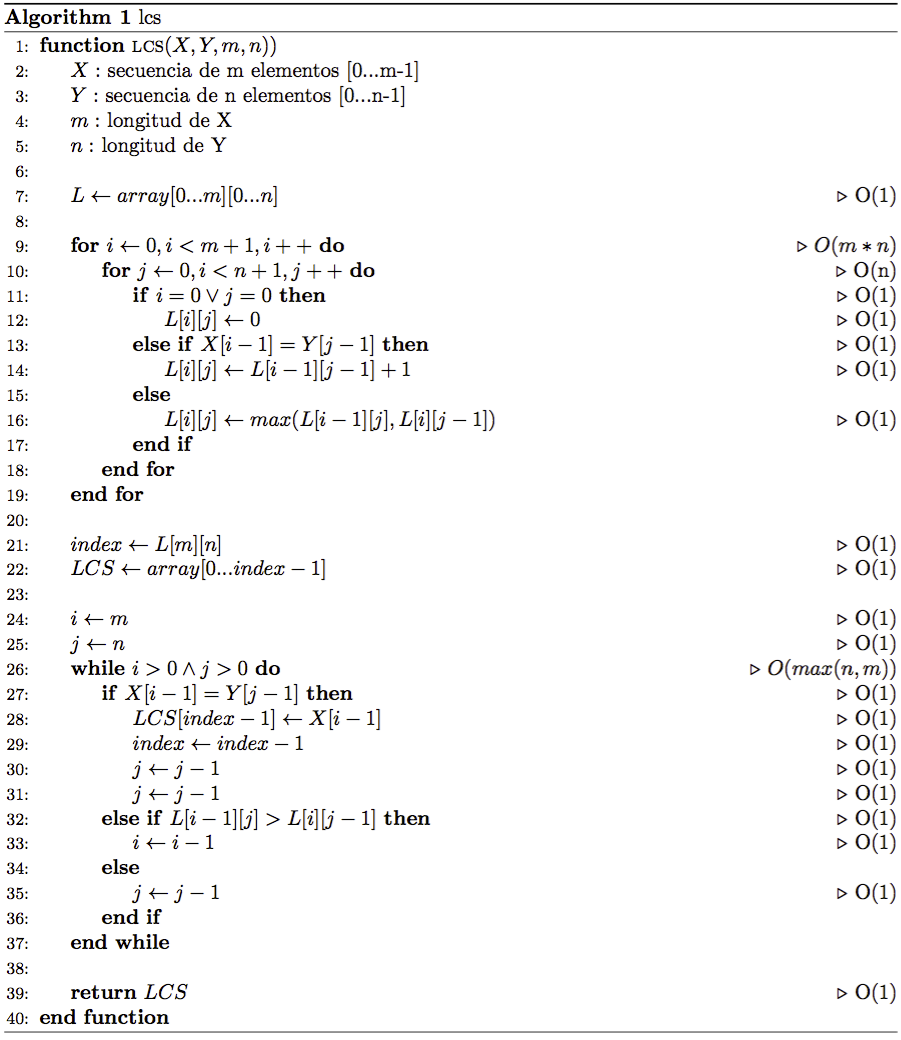
\includegraphics[height=7.5cm]{../res/pseudo_code.png}
					\caption{}
										
					\end{figure}
				\end{frame}
				
				\begin{frame}{Error encontrado}
 			
					\begin{figure}
						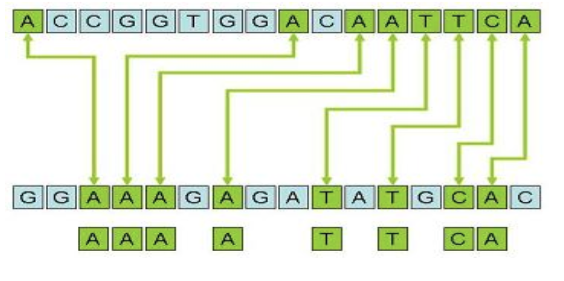
\includegraphics[width=8cm]{../res/imagen.png}
					\caption{}
										
					\end{figure}
				\end{frame}
				
				\begin{frame}{Error encontrado}
 			
				
					\begin{figure}
						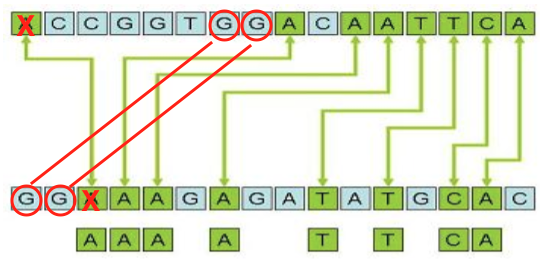
\includegraphics[width=8cm]{../res/imagen_correct.png}
					\caption{}
					
					\end{figure}
				\end{frame}



\section{Fin}


\end{document}
